\documentclass{standalone}
\usepackage{tikz}
\usetikzlibrary{patterns, positioning}


\begin{document}
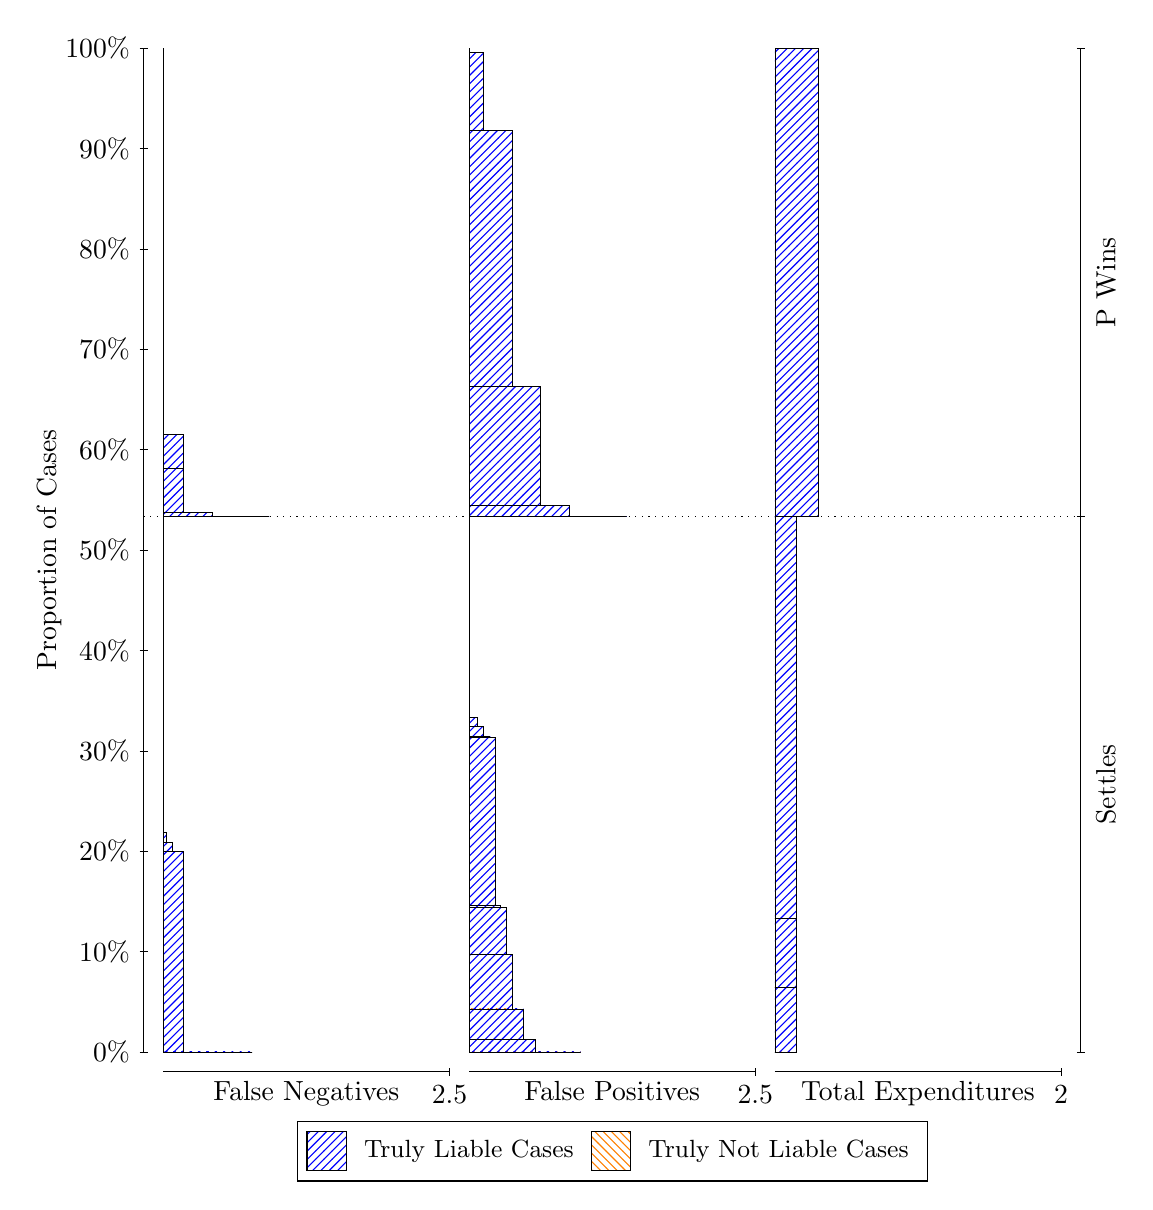
\begin{tikzpicture}
\draw[black, very thin] (1.5,1.75) -- (1.5,14.5);
\node[rotate=90, text=black, anchor=center] at (0.3, 8.125) {Proportion of Cases};
\draw[black, very thin] (1.45,1.75) -- (1.55,1.75);
\node[text=black, anchor=east] at (1.45, 1.75) {0\%};
\draw[black, very thin] (1.45,3.025) -- (1.55,3.025);
\node[text=black, anchor=east] at (1.45, 3.025) {10\%};
\draw[black, very thin] (1.45,4.3) -- (1.55,4.3);
\node[text=black, anchor=east] at (1.45, 4.3) {20\%};
\draw[black, very thin] (1.45,5.575) -- (1.55,5.575);
\node[text=black, anchor=east] at (1.45, 5.575) {30\%};
\draw[black, very thin] (1.45,6.85) -- (1.55,6.85);
\node[text=black, anchor=east] at (1.45, 6.85) {40\%};
\draw[black, very thin] (1.45,8.125) -- (1.55,8.125);
\node[text=black, anchor=east] at (1.45, 8.125) {50\%};
\draw[black, very thin] (1.45,9.4) -- (1.55,9.4);
\node[text=black, anchor=east] at (1.45, 9.4) {60\%};
\draw[black, very thin] (1.45,10.675) -- (1.55,10.675);
\node[text=black, anchor=east] at (1.45, 10.675) {70\%};
\draw[black, very thin] (1.45,11.95) -- (1.55,11.95);
\node[text=black, anchor=east] at (1.45, 11.95) {80\%};
\draw[black, very thin] (1.45,13.225) -- (1.55,13.225);
\node[text=black, anchor=east] at (1.45, 13.225) {90\%};
\draw[black, very thin] (1.45,14.5) -- (1.55,14.5);
\node[text=black, anchor=east] at (1.45, 14.5) {100\%};

\draw[black, very thin] (13.4,1.75) -- (13.4,14.5);
\draw[black, very thin] (13.35,1.75) -- (13.45,1.75);
\node[anchor=west] at (13.35, 1.75) {};
\draw[black, very thin] (13.35,8.548) -- (13.45,8.548);
\node[anchor=west] at (13.35, 8.548) {};
\draw[black, very thin] (13.35,14.5) -- (13.45,14.5);
\node[anchor=west] at (13.35, 14.5) {};

\draw[black, very thin, pattern color=blue, pattern=north east lines] (1.75,1.75) rectangle (2.8763,1.75);
\draw[black, very thin, pattern color=blue, pattern=north east lines] (1.75,1.75) rectangle (2.5857,1.75);
\draw[black, very thin, pattern color=blue, pattern=north east lines] (1.75,1.75) rectangle (2.513,1.75);
\draw[black, very thin, pattern color=blue, pattern=north east lines] (1.75,1.75) rectangle (2.4403,1.75);
\draw[black, very thin, pattern color=blue, pattern=north east lines] (1.75,1.75) rectangle (2.295,1.75);
\draw[black, very thin, pattern color=blue, pattern=north east lines] (1.75,1.75) rectangle (2.2223,1.7502);
\draw[black, very thin, pattern color=blue, pattern=north east lines] (1.75,1.7502) rectangle (2.1497,1.7511);
\draw[black, very thin, pattern color=blue, pattern=north east lines] (1.75,1.7511) rectangle (2.077,1.7511);
\draw[black, very thin, pattern color=blue, pattern=north east lines] (1.75,1.7511) rectangle (2.0043,4.297);
\draw[black, very thin, pattern color=blue, pattern=north east lines] (1.75,4.297) rectangle (1.9317,4.2979);
\draw[black, very thin, pattern color=blue, pattern=north east lines] (1.75,4.2979) rectangle (1.859,4.4112);
\draw[black, very thin, pattern color=blue, pattern=north east lines] (1.75,4.4112) rectangle (1.7863,4.5449);
\draw[black, very thin, pattern color=orange, pattern=north west lines] (1.75,4.5449) rectangle (1.75,4.5449);
\draw[black, very thin, pattern color=blue, pattern=north east lines] (1.75,4.5449) rectangle (1.75,8.548);
\draw[black, very thin, pattern color=blue, pattern=north east lines] (1.75,8.548) rectangle (3.0943,8.548);
\draw[black, very thin, pattern color=blue, pattern=north east lines] (1.75,8.548) rectangle (2.731,8.5482);
\draw[black, very thin, pattern color=blue, pattern=north east lines] (1.75,8.5482) rectangle (2.3677,8.603);
\draw[black, very thin, pattern color=blue, pattern=north east lines] (1.75,8.603) rectangle (2.0043,9.1665);
\draw[black, very thin, pattern color=blue, pattern=north east lines] (1.75,9.1665) rectangle (2.0043,9.5923);
\draw[black, very thin, pattern color=orange, pattern=north west lines] (1.75,9.5923) rectangle (1.75,9.5923);
\draw[black, very thin, pattern color=blue, pattern=north east lines] (1.75,9.5923) rectangle (1.75,14.5);
\draw[black, very thin, pattern color=orange, pattern=north west lines] (5.6333,1.75) rectangle (7.0503,1.75);
\draw[black, very thin, pattern color=blue, pattern=north east lines] (5.6333,1.75) rectangle (7.0503,1.75);
\draw[black, very thin, pattern color=orange, pattern=north west lines] (5.6333,1.75) rectangle (6.7597,1.75);
\draw[black, very thin, pattern color=blue, pattern=north east lines] (5.6333,1.75) rectangle (6.7597,1.75);
\draw[black, very thin, pattern color=blue, pattern=north east lines] (5.6333,1.75) rectangle (6.687,1.7523);
\draw[black, very thin, pattern color=orange, pattern=north west lines] (5.6333,1.7523) rectangle (6.6143,1.7523);
\draw[black, very thin, pattern color=blue, pattern=north east lines] (5.6333,1.7523) rectangle (6.6143,1.7523);
\draw[black, very thin, pattern color=orange, pattern=north west lines] (5.6333,1.7523) rectangle (6.469,1.7523);
\draw[black, very thin, pattern color=blue, pattern=north east lines] (5.6333,1.7523) rectangle (6.469,1.9123);
\draw[black, very thin, pattern color=blue, pattern=north east lines] (5.6333,1.9123) rectangle (6.3963,1.9133);
\draw[black, very thin, pattern color=blue, pattern=north east lines] (5.6333,1.9133) rectangle (6.3237,2.2963);
\draw[black, very thin, pattern color=blue, pattern=north east lines] (5.6333,2.2963) rectangle (6.251,2.2965);
\draw[black, very thin, pattern color=orange, pattern=north west lines] (5.6333,2.2965) rectangle (6.1783,2.2965);
\draw[black, very thin, pattern color=blue, pattern=north east lines] (5.6333,2.2965) rectangle (6.1783,2.9862);
\draw[black, very thin, pattern color=blue, pattern=north east lines] (5.6333,2.9862) rectangle (6.1057,3.5876);
\draw[black, very thin, pattern color=blue, pattern=north east lines] (5.6333,3.5876) rectangle (6.033,3.609);
\draw[black, very thin, pattern color=blue, pattern=north east lines] (5.6333,3.609) rectangle (5.9603,5.7529);
\draw[black, very thin, pattern color=blue, pattern=north east lines] (5.6333,5.7529) rectangle (5.8877,5.7531);
\draw[black, very thin, pattern color=blue, pattern=north east lines] (5.6333,5.7531) rectangle (5.815,5.8868);
\draw[black, very thin, pattern color=blue, pattern=north east lines] (5.6333,5.8868) rectangle (5.7423,6.0001);
\draw[black, very thin, pattern color=blue, pattern=north east lines] (5.6333,6.0001) rectangle (5.6697,6.0011);
\draw[black, very thin, pattern color=blue, pattern=north east lines] (5.6333,6.0011) rectangle (5.6333,8.548);
\draw[black, very thin, pattern color=orange, pattern=north west lines] (5.6333,8.548) rectangle (7.6317,8.548);
\draw[black, very thin, pattern color=blue, pattern=north east lines] (5.6333,8.548) rectangle (7.6317,8.548);
\draw[black, very thin, pattern color=orange, pattern=north west lines] (5.6333,8.548) rectangle (7.2683,8.548);
\draw[black, very thin, pattern color=blue, pattern=north east lines] (5.6333,8.548) rectangle (7.2683,8.5498);
\draw[black, very thin, pattern color=orange, pattern=north west lines] (5.6333,8.5498) rectangle (6.905,8.5498);
\draw[black, very thin, pattern color=blue, pattern=north east lines] (5.6333,8.5498) rectangle (6.905,8.6873);
\draw[black, very thin, pattern color=orange, pattern=north west lines] (5.6333,8.6873) rectangle (6.5417,8.6873);
\draw[black, very thin, pattern color=blue, pattern=north east lines] (5.6333,8.6873) rectangle (6.5417,10.198);
\draw[black, very thin, pattern color=orange, pattern=north west lines] (5.6333,10.198) rectangle (6.1783,10.198);
\draw[black, very thin, pattern color=blue, pattern=north east lines] (5.6333,10.198) rectangle (6.1783,13.456);
\draw[black, very thin, pattern color=blue, pattern=north east lines] (5.6333,13.456) rectangle (5.815,14.445);
\draw[black, very thin, pattern color=blue, pattern=north east lines] (5.6333,14.445) rectangle (5.6333,14.5);
\draw[black, very thin, pattern color=orange, pattern=north west lines] (9.5167,1.75) rectangle (9.7892,1.75);
\draw[black, very thin, pattern color=blue, pattern=north east lines] (9.5167,1.75) rectangle (9.7892,2.5744);
\draw[black, very thin, pattern color=orange, pattern=north west lines] (9.5167,2.5744) rectangle (9.7892,2.5744);
\draw[black, very thin, pattern color=blue, pattern=north east lines] (9.5167,2.5744) rectangle (9.7892,3.4493);
\draw[black, very thin, pattern color=orange, pattern=north west lines] (9.5167,3.4493) rectangle (9.7892,3.4493);
\draw[black, very thin, pattern color=blue, pattern=north east lines] (9.5167,3.4493) rectangle (9.7892,8.548);
\draw[black, very thin, pattern color=orange, pattern=north west lines] (9.5167,8.548) rectangle (10.062,8.548);
\draw[black, very thin, pattern color=blue, pattern=north east lines] (9.5167,8.548) rectangle (10.062,14.5);
\draw[black, dotted] (1.5,8.548) -- (13.4,8.548);
\draw[black, very thin] (1.75,1.5) -- (5.3833,1.5);
\node[text=black, anchor=north] at (3.5667, 1.5) {False Negatives};
\draw[black, very thin] (5.3833,1.45) -- (5.3833,1.55);
\node[text=black, anchor=north] at (5.3833, 1.45) {2.5};

\draw[black, very thin] (5.6333,1.5) -- (9.2667,1.5);
\node[text=black, anchor=north] at (7.45, 1.5) {False Positives};
\draw[black, very thin] (9.2667,1.45) -- (9.2667,1.55);
\node[text=black, anchor=north] at (9.2667, 1.45) {2.5};

\draw[black, very thin] (9.5167,1.5) -- (13.15,1.5);
\node[text=black, anchor=north] at (11.333, 1.5) {Total Expenditures};
\draw[black, very thin] (13.15,1.45) -- (13.15,1.55);
\node[text=black, anchor=north] at (13.15, 1.45) {2};

\node[text=black, centered, rotate=90] at (13.72, 5.149) {Settles};
\node[text=black, centered, rotate=90] at (13.72, 11.524) {P Wins};

\draw (7.449999999999999,1.5) node[draw=none] (baseCoordinate) {};
\begin{scope}[align=center]
        \matrix[scale=0.5, draw=black, below=0.5cm of baseCoordinate, nodes={draw}, column sep=0.1cm]{
            \node[rectangle, draw, minimum width=0.5cm, minimum height=0.5cm, pattern color=blue, pattern=north east lines] {}; &
            \node[draw=none, font=\small, text=black] (B) {Truly Liable Cases}; &
            \node[rectangle, draw, minimum width=0.5cm, minimum height=0.5cm, pattern color=orange, pattern=north west lines] {}; &
            \node[draw=none, font=\small, text=black] (B) {Truly Not Liable Cases}; \\
            };
\end{scope}

\end{tikzpicture}
\end{document}